\documentclass[a4paper,14pt]{extarticle}

\newcommand{\stend}{\textbf{Wb-demo-kit v.2}}

% Путь до папки с общими шаблонами
\newcommand{\pathToCommonFolder}{/home/denilai/Documents/repos/latex/Common}

% Название работы в титуле
\newcommand{\workname}{Отчет по лабораторной работе № 6}
% Название дисциплины в титуле
\newcommand{\discipline}{Инструментальные средства разработки
	вычислительных систем}
% Название кафедры в титуле
\newcommand{\kafedra}{Кафедра вычислительной техники}
% Тема работы в титуле
\newcommand{\theme}{Межпроцессное
	взаимодействие}
% Должность преподавателя в титуле
\newcommand{\rang}{}

% ФИО студента в титуле
\newcommand{\studentfio}{К.~Ю.~Денисов}%\\Д.~Н.~Федосеев\\А.~М.~Сосунов}\\%К.~Ю.~Денисов\\%И.~А.~Кремнев
% ФИО преподавателя в титуле
\newcommand{\teacherfio}{И.~Р.~Сон}


\usepackage{tabularx}
\usepackage{lastpage}


\usepackage{booktabs}
\newcolumntype{b}{X}
\newcolumntype{s}{>{\hsize=.5\hsize}X}
\newcommand{\heading}[1]{\multicolumn{1}{|c|}{#1}}

% установка размера шрифта для всего документа
%\fontsize{20pt}{18pt}\selectfont
\usepackage{extsizes} % Возможность сделать 14-й шрифт

% Вставка заготовки преамбулы
% Этот шаблон документа разработан в 2014 году
% Данилом Фёдоровых (danil@fedorovykh.ru) 
% для использования в курсе 
% <<Документы и презентации в \LaTeX>>, записанном НИУ ВШЭ
% для Coursera.org: http://coursera.org/course/latex .
% Исходная версия шаблона --- 
% https://www.writelatex.com/coursera/latex/5.3

% В этом документе преамбула

% Для корректного использования русских символов в формулах
% пакеты hyperref и настройки, связанные с ним, стоит загуржать
% перед загрузкой пакета mathtext



% поддержка русских букв
% кодировка шрифта
%\usepackage[T2A]{fontenc} 
\usepackage{pscyr}

% использование ненумеровонного абзаца с добавлением его в содержаниеl

\newcommand{\anonsection}[1]{\section*{#1}\addcontentsline{toc}{section}{#1}}
\newcommand{\sectionunderl}[1]{\section*{\underline{#1}}}


% настройка окружения enumerate
\usepackage{enumitem}
\setlist{noitemsep}
\setlist[enumerate]{labelsep=*, leftmargin=1.5pc}

\usepackage{hyperref}

% сначала ставить \usepackage{extsizes} % Возможность сделать 14-й шрифт
% для корректной установки полей вставлять преамбулу следует в последнюю очередь (но перед дерективой замены \rmdefault)
\usepackage[top=20mm,bottom=25mm,left=35mm,right=20mm]{geometry} % Простой способ задавать поля

\hypersetup{				% Гиперссылки
	unicode=true,           % русские буквы в раздела PDF
	pdftitle={Заголовок},   % Заголовок
	pdfauthor={Автор},      % Автор
	pdfsubject={Тема},      % Тема
	pdfcreator={Создатель}, % Создатель
	pdfproducer={Производитель}, % Производитель
	pdfkeywords={keyword1} {key2} {key3}, % Ключевые слова
	colorlinks=true,       	% false: ссылки в рамках; true: цветные ссылки
	linkcolor=red,          % внутренние ссылки
	citecolor=black,        % на библиографию
	filecolor=magenta,      % на файлы
	urlcolor=blue           % на URL
}

%%% Работа с русским языком
\usepackage{cmap}					% поиск в PDF
\usepackage{mathtext} 				% русские буквы в формулах
\usepackage[T2A]{fontenc}			% кодировка
\usepackage[utf8]{inputenc}			% кодировка исходного текста
\usepackage[english,russian]{babel}	% локализация и переносы
\usepackage{indentfirst}
\frenchspacing

%для изменения названия списка иллюстраций
\usepackage{tocloft}


\renewcommand{\epsilon}{\ensuremath{\varepsilon}}
\renewcommand{\phi}{\ensuremath{\varphi}}
\renewcommand{\kappa}{\ensuremath{\varkappa}}
\renewcommand{\le}{\ensuremath{\leqslant}}
\renewcommand{\leq}{\ensuremath{\leqslant}}
\renewcommand{\ge}{\ensuremath{\geqslant}}
\renewcommand{\geq}{\ensuremath{\geqslant}}
\renewcommand{\emptyset}{\varnothing}

% Изменения параметров списка иллюстраций
\renewcommand{\cftfigfont}{Рисунок } % добавляем везде "Рисунок" перед номером
\addto\captionsrussian{\renewcommand\listfigurename{Список иллюстративного материала}}

\newcommand{\tm}{\texttrademark\ }
\newcommand{\reg}{\textregistered\ }


%%% Дополнительная работа с математикой
\usepackage{amsmath,amsfonts,amssymb,amsthm,mathtools} % AMS
\usepackage{icomma} % "Умная" запятая: $0,2$ --- число, $0, 2$ --- перечисление

%% Номера формул
%\mathtoolsset{showonlyrefs=true} % Показывать номера только у тех формул, на которые есть \eqref{} в тексте.
%\usepackage{leqno} % Нумереация формул слева

%% Свои команды
\DeclareMathOperator{\sgn}{\mathop{sgn}}

%% Перенос знаков в формулах (по Львовскому)
\newcommand*{\hm}[1]{#1\nobreak\discretionary{}
{\hbox{$\mathsurround=0pt #1$}}{}}


% отступ для первого абзаца главы или параграфа
%\usepackage{indentfirst}

%%% Работа с картинками
\usepackage{graphicx}  % Для вставки рисунков
\graphicspath{{images/}{screnshots/}}  % папки с картинками
\DeclareGraphicsExtensions{.pdf,.png,.jpg}
\setlength\fboxsep{3pt} % Отступ рамки \fbox{} от рисунка
\setlength\fboxrule{1pt} % Толщина линий рамки \fbox{}
\usepackage{wrapfig} % Обтекание рисунков текстом

%%% Работа с таблицами
\usepackage{array,tabularx,tabulary,booktabs} % Дополнительная работа с таблицами
\usepackage{longtable}  % Длинные таблицы
\usepackage{multirow} % Слияние строк в таблице

%%% Теоремы
\theoremstyle{plain} % Это стиль по умолчанию, его можно не переопределять.
\newtheorem{theorem}{Теорема}[section]
\newtheorem{proposition}[theorem]{Утверждение}

\theoremstyle{plain} % Это стиль по умолчанию, его можно не переопределять.
\newtheorem{work}{Практическая работа}[part]


 
 
\theoremstyle{definition} % "Определение"
\newtheorem{corollary}{Следствие}[theorem]
\newtheorem{problem}{Задача}[section]
 
\theoremstyle{remark} % "Примечание"
\newtheorem*{nonum}{Решение}



%%% Программирование
\usepackage{etoolbox} % логические операторы

%%% Страница

%	\usepackage{fancyhdr} % Колонтитулы
% 	\pagestyle{fancy}
%   \renewcommand{\headrulewidth}{0pt}  % Толщина линейки, отчеркивающей верхний колонтитул
% 	\lfoot{Нижний левый}
% 	\rfoot{Нижний правый}
% 	\rhead{Верхний правый}
% 	\chead{Верхний в центре}
% 	\lhead{Верхний левый}
%	\cfoot{Нижний в центре} % По умолчанию здесь номер страницы

\usepackage{setspace} % Интерлиньяж
\onehalfspacing % Интерлиньяж 1.5
%\doublespacing % Интерлиньяж 2
%\singlespacing % Интерлиньяж 1

\usepackage{lastpage} % Узнать, сколько всего страниц в документе.

\usepackage{soul} % Модификаторы начертания


\usepackage[usenames,dvipsnames,svgnames,table,rgb]{xcolor}


\usepackage{csquotes} % Еще инструменты для ссылок

%\usepackage[style=authoryear,maxcitenames=2,backend=biber,sorting=nty]{biblatex}

\usepackage{multicol} % Несколько колонок

\usepackage{tikz} % Работа с графикой
\usepackage{pgfplots}
\usepackage{pgfplotstable}

% модуль для вставки рыбы
\usepackage{blindtext}

\usepackage{listings}
\usepackage{color}


% для поворота отдельной страницы. Использовать окружение \landscape
\usepackage{pdflscape} 
\usepackage{rotating} 


\definecolor{mygreen}{rgb}{0,0.6,0}
\definecolor{mygray}{rgb}{0.5,0.5,0.5}
\definecolor{mymauve}{rgb}{0.58,0,0.82}


% пример импорта файла
%\lstinputlisting{/home/denilai/repomy/conf/distributions}

\lstset{
	language=Python,
	basicstyle=\footnotesize,        % the size of the fonts that are used for the code
	numbers=left,                    % where to put the line-numbers; possible values are (none, left, right)
	numbersep=5pt,                   % how far the line-numbers are from the code
	numberstyle=\tiny\color{mygray}, % the style that is used for the line-numbers
	stepnumber=2,                    % the step between two line-numbers. If it's 1, each line will be numbered
	% Tab - 2 пробела
	tabsize=2,    
	% Автоматический перенос строк
	breaklines=true,
	frame=single,
	breakatwhitespace=true,
	title=\lstname 
}





\setcounter{withouttheme}{0}
\setcounter{withoutsubmissiondate}{1}


%если нужна тема работы в отчете, то указать в скобках 0, иначе 1
%\setcounter{withouttheme}{0}
%если нужна дата представления отчета, то указать в скобках 0, иначе 1
%\setcounter{\withoutsubmissiondate}{0}

% установка полуторного интервала
% \usepackage{setspace}  
% \onehalfspacing

% использовать Times New Roman
\renewcommand{\rmdefault}{ftm}


\newcommand{\tb}{ThingsBoard~}

\begin{document}
	\thispagestyle{empty}
	% Вставка первого титульного листа
	% Есть две версии титульного листа - одиночный (titul) и групповой (titulAll)
	%\newcounter{withouttheme}

%\setcounter{withouttheme}{<n>} установить значение счетчика  withouttheme для определения, нужна ли тема
%    {0} - нужна
%    {1} - не нужна

%\setcounter{withoutsubmissiondate}{<n>} установить значение счетчика  withoutsubmissiondate для определения, нужна ли дата представления к защите
%     {0} - нужна
%     {1} - не нужена
\begin{center}
	\begin{figure}[h!]
		\begin{center}
		%\vspace{-10ex}
		
\includegraphics[width=0.17\linewidth]{\pathToCommonFolder/gerb}
		%\caption{}\label{pic:first}
		%	\vspace{5ex}
		\end{center}	
	\end{figure}
 	\small	МИНОБРНАУКИ РОССИИ \\
	Федеральное государственное бюджетное образовательное учреждение\\
						высшего образования\\
\normalsize					
\textbf{«МИРЭА – Российский технологический университет»\\
						РТУ МИРЭА}\\
						\noindent\rule{1\linewidth}{1pt}\\
       Институт информационных технологий\\ %\vspace{2ex}
					\kafedra\\
		\vspace{3ex}
			\large \textbf{\workname}  \\
		%\vspace{1ex}
						по дисциплине\\ «\discipline» \\
		\vspace{3ex}
		\ifnum \value{withouttheme}=0 {
			\textbf{Тема работы:}\\ <<\theme>>
		}
		\else {}
		\fi
\vspace{10ex}
\small
\begin{table}[h!]
\begin{tabular}{lp{0.6\linewidth}l}
	\textbf{Выполнил:} & студент группы ИВБО-02-19 & \\ 
	& & \studentfio \\%Д.~Н.~Федосеев\\%А.~М.~Сосунов\\%К.~Ю.~Денисов\\%И.~А.~Кремнев
	\textbf{Принял:} & \rang & \\
	& & \teacherfio \hfill\\
\end{tabular}
\end{table}
\end{center}
\ifnum \value{withoutsubmissiondate}=0 {
	\begin{flushleft}
		Работа представлена к защите <<\rule{3ex}{1pt}>>\rule{10ex}{1pt} 202\rule{1ex}{1pt} г.\hfill
	\end{flushleft}
\else {}
\fi

\normalsize
\begin{center}	
\vfill
Москва 2022
\end{center}

	\newpage
	\tableofcontents
	\newpage
	%\listoftables
	
\normalsize


\section{Цель работы}
Изучить способы межпроцессного взаимодействия в UNIX-системах.

\section{Задание}
Написать программы, демонстрирующие реализацию межпроцессное взаимодействие с помощью:
\begin{itemize}
	\item каналов (pipes);
	\item семафоров (semaphores);
	\item очередей сообщений (message queries);
	\item сегментов разделяемой памяти.
\end{itemize}

\section{Ход работы}

\subsection{Каналы}

Напишем программу, демонстрирующую организацию межпроцессного взаимодействия с помощью каналов. Исходный код приведен в листинге \ref{lst:pipes}.

\begin{lstlisting}[language=C, caption={pipes.c}, label={lst:pipes}]
#include <stdio.h>
#include <unistd.h>
#include <stdlib.h>
#include <string.h>
#include <sys/types.h>


int main(void)
{
	int fd[2], nbytes;
	char string[] = "IPC organized successfully!\n";
	char readbuffer[80]; 
	pipe(fd);
	pid_t childpid;
	childpid = fork();
	if(childpid == -1)
	{
		perror("fork creation");
		exit(1);
	}

	if(childpid == 0)
	{
		/* Child process close read file descriptor  */ 
		close(fd[0]);
		write(fd[1], string, (strlen(string)+1));
		exit(0);
	}
	else
	{
		/* Parrent process close write file desriptor */ 
		close(fd[1]);
		/* Read string from pipe */ 
		nbytes = read(fd[0], readbuffer, sizeof(readbuffer)); 
		printf("The string received from the process %d: %s", childpid, readbuffer);
	}
	return(0);
}
\end{lstlisting}

Данная программа создает дочерний процесс, который использует ранее созданный канал для отправления строки родительскому.

Скомпилируем программу с помощью команды \texttt{\$ gcc pipes.c -o pipes}. Вывод программы приведен на рисунке \ref{fig:pipes}.

% TODO: \usepackage{graphicx} required
\begin{figure}[h!]
	\centering
	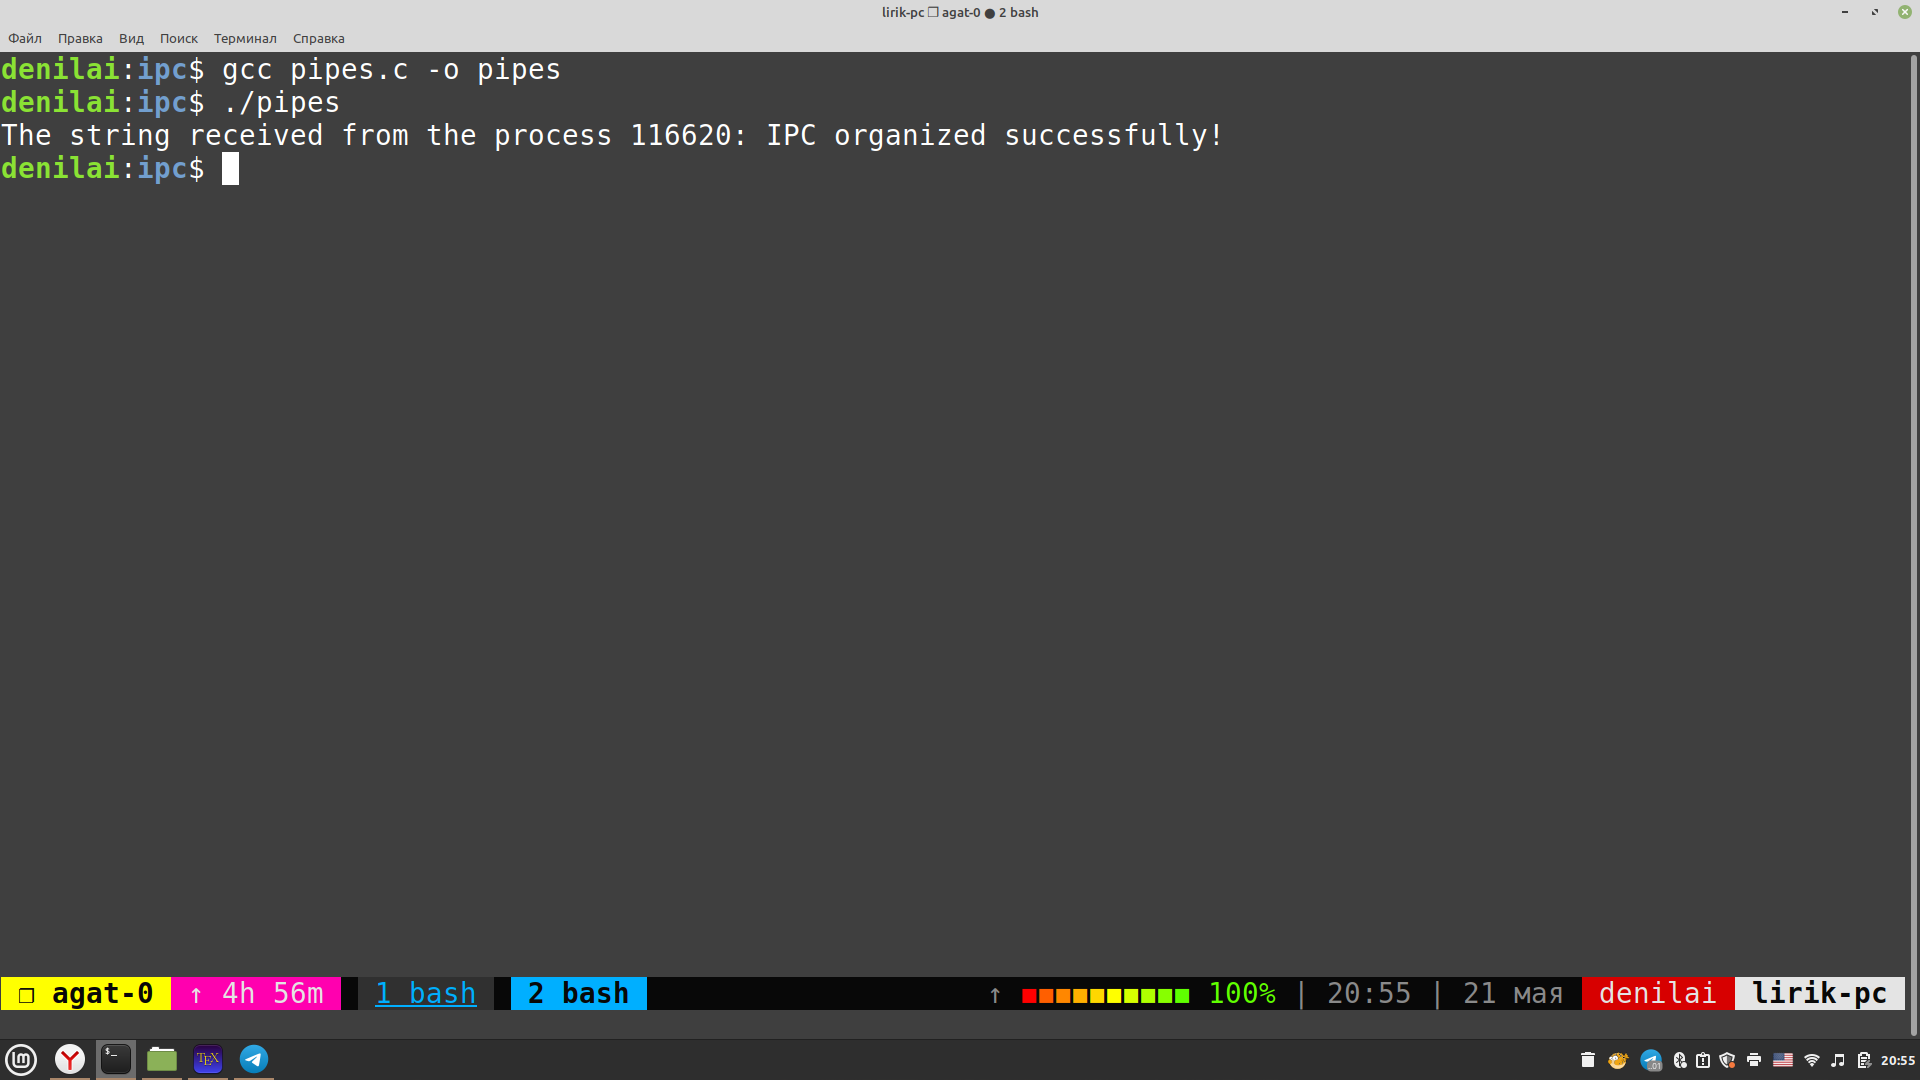
\includegraphics[width=0.9\linewidth]{images/6/pipes}
	\caption{Вывод программы pipes}
	\label{fig:pipes}
\end{figure}

Программа работает корректно. 

\subsection{Семафоры}

Напишем программу, демонстрирующую организацию межпроцессного взаимодействия с помощью семафоров. Работать будем с семафорами в соответствии с POSIX API. 

Исходный код приведен в листинге \ref{lst:sems}.


\begin{lstlisting}[language=C, caption={sems.c}, label={lst:sems}]
#include <stdio.h>
#include <pthread.h>
#include <semaphore.h>
#include <unistd.h>
#include <stdlib.h>

sem_t sem;

void* first(void* arg)
{
	FILE *fp;
	//wait
	sem_wait(&sem);
	printf("\nSeizing control of the semaphore\n");
	
	//critical section
	sleep(4);
	if ((fp=fopen("semtest.txt", "a")) == NULL){
		perror("posixsem.fopen");
		exit(1);
	}
	fputs("Caprture file for write. Thread 1\n", fp);
	fclose(fp);
	
	printf("\nTransfer of control over the semaphore\n");
	sem_post(&sem);
}

void* second(void* arg)
{
	FILE *fp;
	//wait
	sem_wait(&sem);
	printf("\nSeizing control of the semaphore\n");
	
	//critical section
	sleep(4);
	if ((fp=fopen("semtest.txt", "a")) == NULL){
		perror("posixsem.fopen");
		exit(1);
	}
	fputs("Caprture file for write. Thread 2\n", fp);
	fclose(fp);
	
	printf("\nTransfer of control over the semaphore\n");
	sem_post(&sem);
}


int main()
{
	sem_init(&sem, 0, 1);
	pthread_t t1,t2;
	pthread_create(&t1,NULL,first,NULL);
	
	pthread_create(&t2,NULL,second,NULL);
	pthread_join(t1,NULL);
	pthread_join(t2,NULL);
	sem_destroy(&sem);
	return 0;
}

\end{lstlisting}

В данном примере создаются потоки, в качестве start\_routine которых выступают функции first и second. Потоки запрашивают доступ к семафору, чтобы указать на то, что далее следует обращение к разделяемому ресурсу --- файлу. 

В коде используются два метода -- pthread\_crate() и pthread\_join().

\begin{lstlisting}[language=C]

#define _OPEN_THREADS
#include <pthread.h>


int pthread_create(pthread_t *thread, pthread_attr_t *attr,
					void *(*start_routine) (void *arg), void *arg);

\end{lstlisting}

Создает новый поток внутри процесса с атрибутами, определенными объектом атрибута потока attr, который создается pthread\_attr\_init().

Если значение attr равно NULL, используются атрибуты по умолчанию. 

pthread\_t --- это тип данных, используемый для уникальной идентификации потока. Он возвращается функцией pthread\_create() и используется приложением в вызовах функций, требующих идентификатора потока.

Поток создается под управлением start\_routine с единственным аргументом arg. Если функция pthread\_create() завершится успешно, поток будет содержать идентификатор созданного потока. В случае сбоя новый поток не создается, а содержимое местоположения, на которое ссылается поток, не определено.


Максимальное количество потоков зависит от размера частной области ниже 16M. pthread\_create() проверяет это адресное пространство перед созданием нового потока. Реалистичный предел составляет от 200 до 400 потоков.

\begin{lstlisting}[language=C]

#define _OPEN_THREADS
#include <pthread.h>


int pthread_join(pthread_t thread, void **status);


\end{lstlisting}

Позволяет вызывающему потоку дождаться окончания целевого потока.


Скомпилируем программу с помощью команды \texttt{\$ gcc posix.sem.c -lpthread -lrt -o sems} и запустим исполнимый файл \texttt{./sems}. После завершения работы программы выведем содержание файла semtest.txt (см. рисунок \ref{fig:sems}).

% TODO: \usepackage{graphicx} required
\begin{figure}[h!]
	\centering
	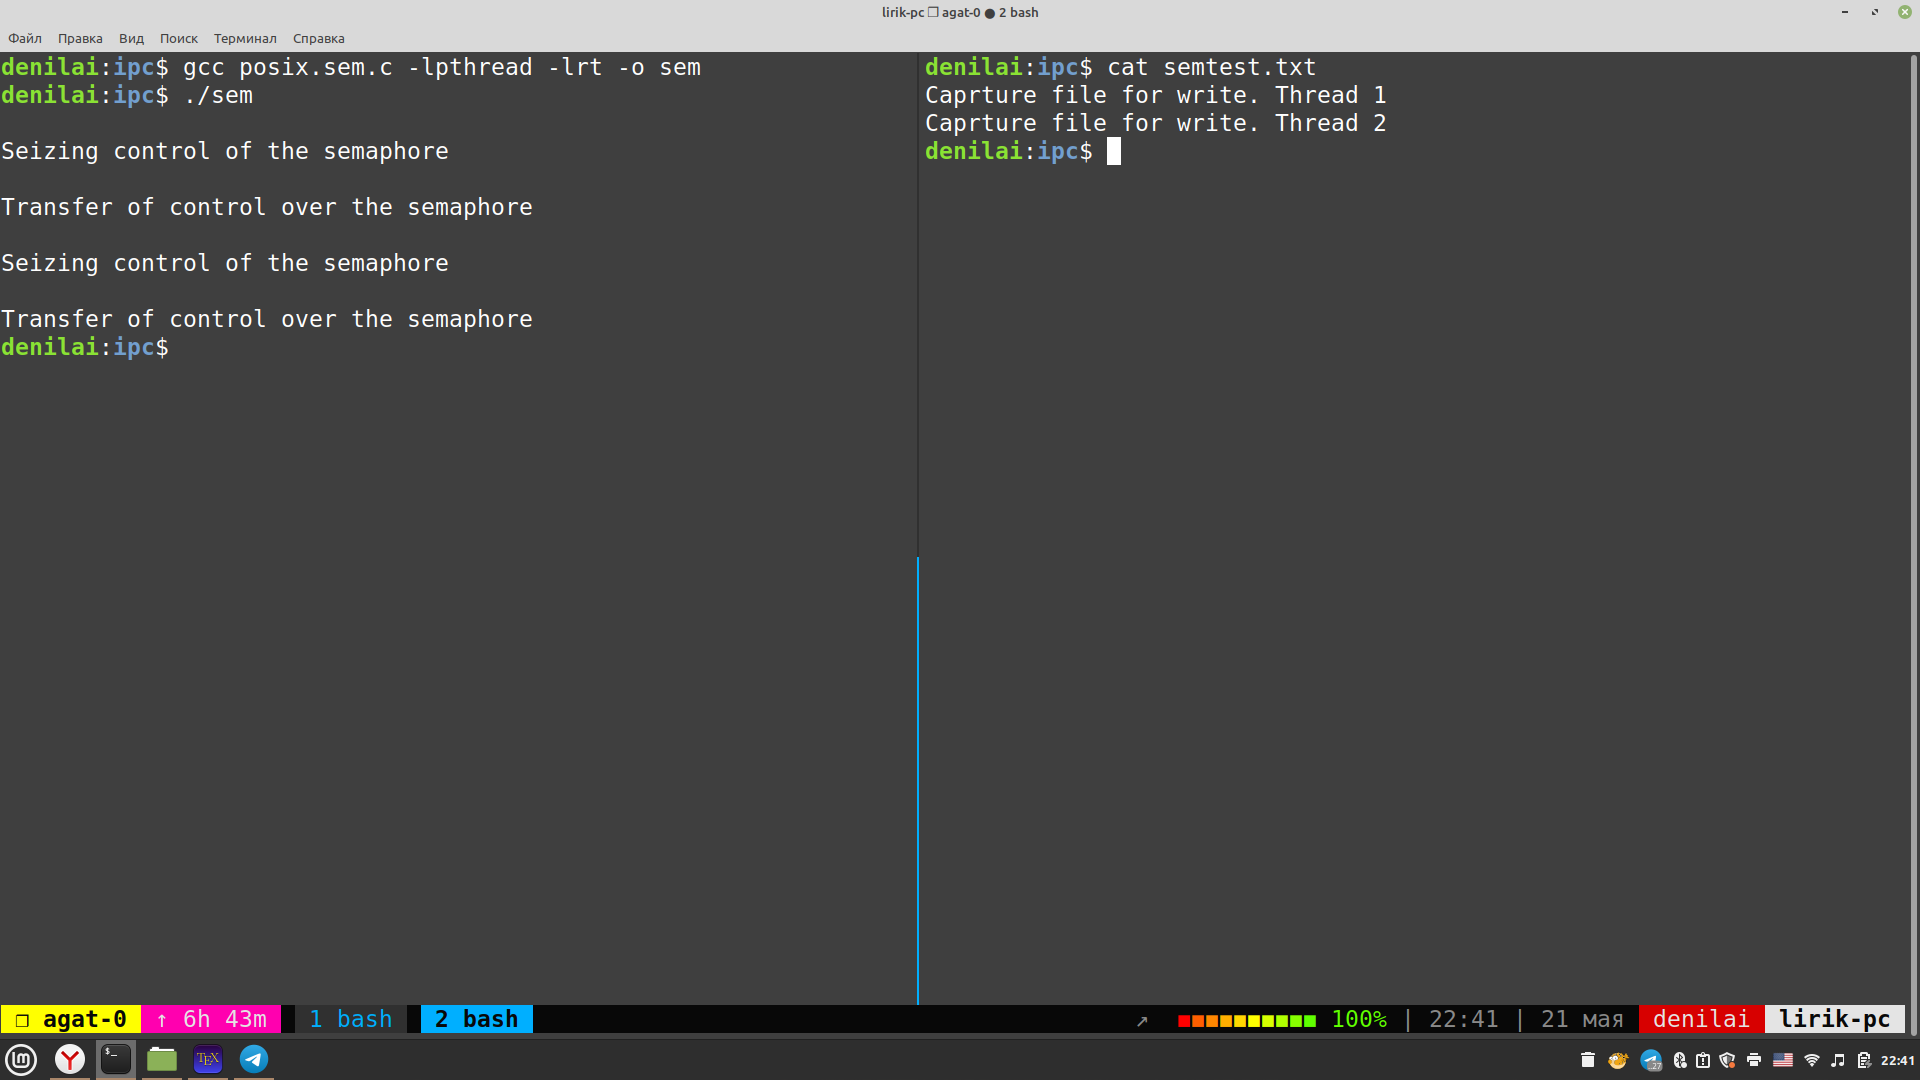
\includegraphics[width=0.9\linewidth]{images/6/sems}
	\caption{Вывод программы sems}
	\label{fig:sems}
\end{figure}

\subsection{Именованные каналы}

Напишем программу, демонстрирующую организацию межпроцессного взаимодействия с помощью именованных каналов. Именованный канал (pipe) позволяет взаимодействовать двум не родственным процессам. 
 
Реализуем модель взаимодействия отправитель-получатель. 

Создадим файл npipesender.c, в котором опишем процесс отправки строковой переменной в именованный канал "npipe". В файле npipereceiver.c опишем процесс получения сообщений, переданных через канал "npipe".

\begin{lstlisting}[language=C, caption={npipereceiver.c}, label={lst:npiper}]
	#include <stdio.h>
	#include <stdlib.h>
	#include <sys/stat.h>
	#include <unistd.h>
	
	#define NPIPE_FILE "npipe"
	#define BUFF_SIZE 80
	
	int main(void)
	{
		FILE *fp;
		char readbuf[80];
		
		/* Create the NPIPE if it does not exist */
		umask(0);
		/* int mknod(char *pathname, int mode, int dev);
		Constant S_IFIFO from <sys/stat.h> */
		unlink(NPIPE_FILE);
		mknod(NPIPE_FILE, S_INPIPE|0666, 0);
		
		while(1)
		{
			if((fp = fopen(NPIPE_FILE, "r")) == NULL){
				perror("npipeserver.fopen");
			}
			fgets(readbuf, BUFF_SIZE, fp);
			printf("Received string: %s\n", readbuf);
			fclose(fp);
		}
	
	return(0);
	}
	
\end{lstlisting}


\begin{lstlisting}[language=C, caption={npipesender.c}, label={lst:npipes}]
#include <stdio.h>
#include <stdlib.h>
#include <sys/stat.h>
#include <unistd.h>

#define NPIPE_FILE "myFifo"
#define BUFF_SIZE 80

int main(void)
{
	FILE *fp;
	char readbuf[80];
	
	/* Create the NPIPE if it does not exist */
	umask(0);
	/* int mknod(char *pathname, int mode, int dev);
	 Constant S_IFIFO from <sys/stat.h> */
	unlink(NPIPE_FILE);
	mknod(NPIPE_FILE, S_INPIPE|0666, 0);
	
	while(1)
	{
		if((fp = fopen(NPIPE_FILE, "r")) == NULL){
			perror("npipeserver.fopen");
		}
		fgets(readbuf, BUFF_SIZE, fp);
		printf("Received string: %s\n", readbuf);
		fclose(fp);
	}
	
	return(0);
}

\end{lstlisting}


Скомпилируем файлы с помощью команды \texttt{\$ gcc npipesender.c -o npipesender; gcc npipereceiver.c -o npipereceiver}.

Для того, чтобы удостовериться в правильной работе программ, запустим npipereceiver в фоновом режиме командой \texttt{\$ ./npipereceiver \&}. В отдельном окне будем запускать программу \texttt{./npipesender } со строковым аргументом -- отправляемым сообщением (см. рисунок \ref{fig:demo}).

% TODO: \usepackage{graphicx} required
\begin{figure}[h!]
	\centering
	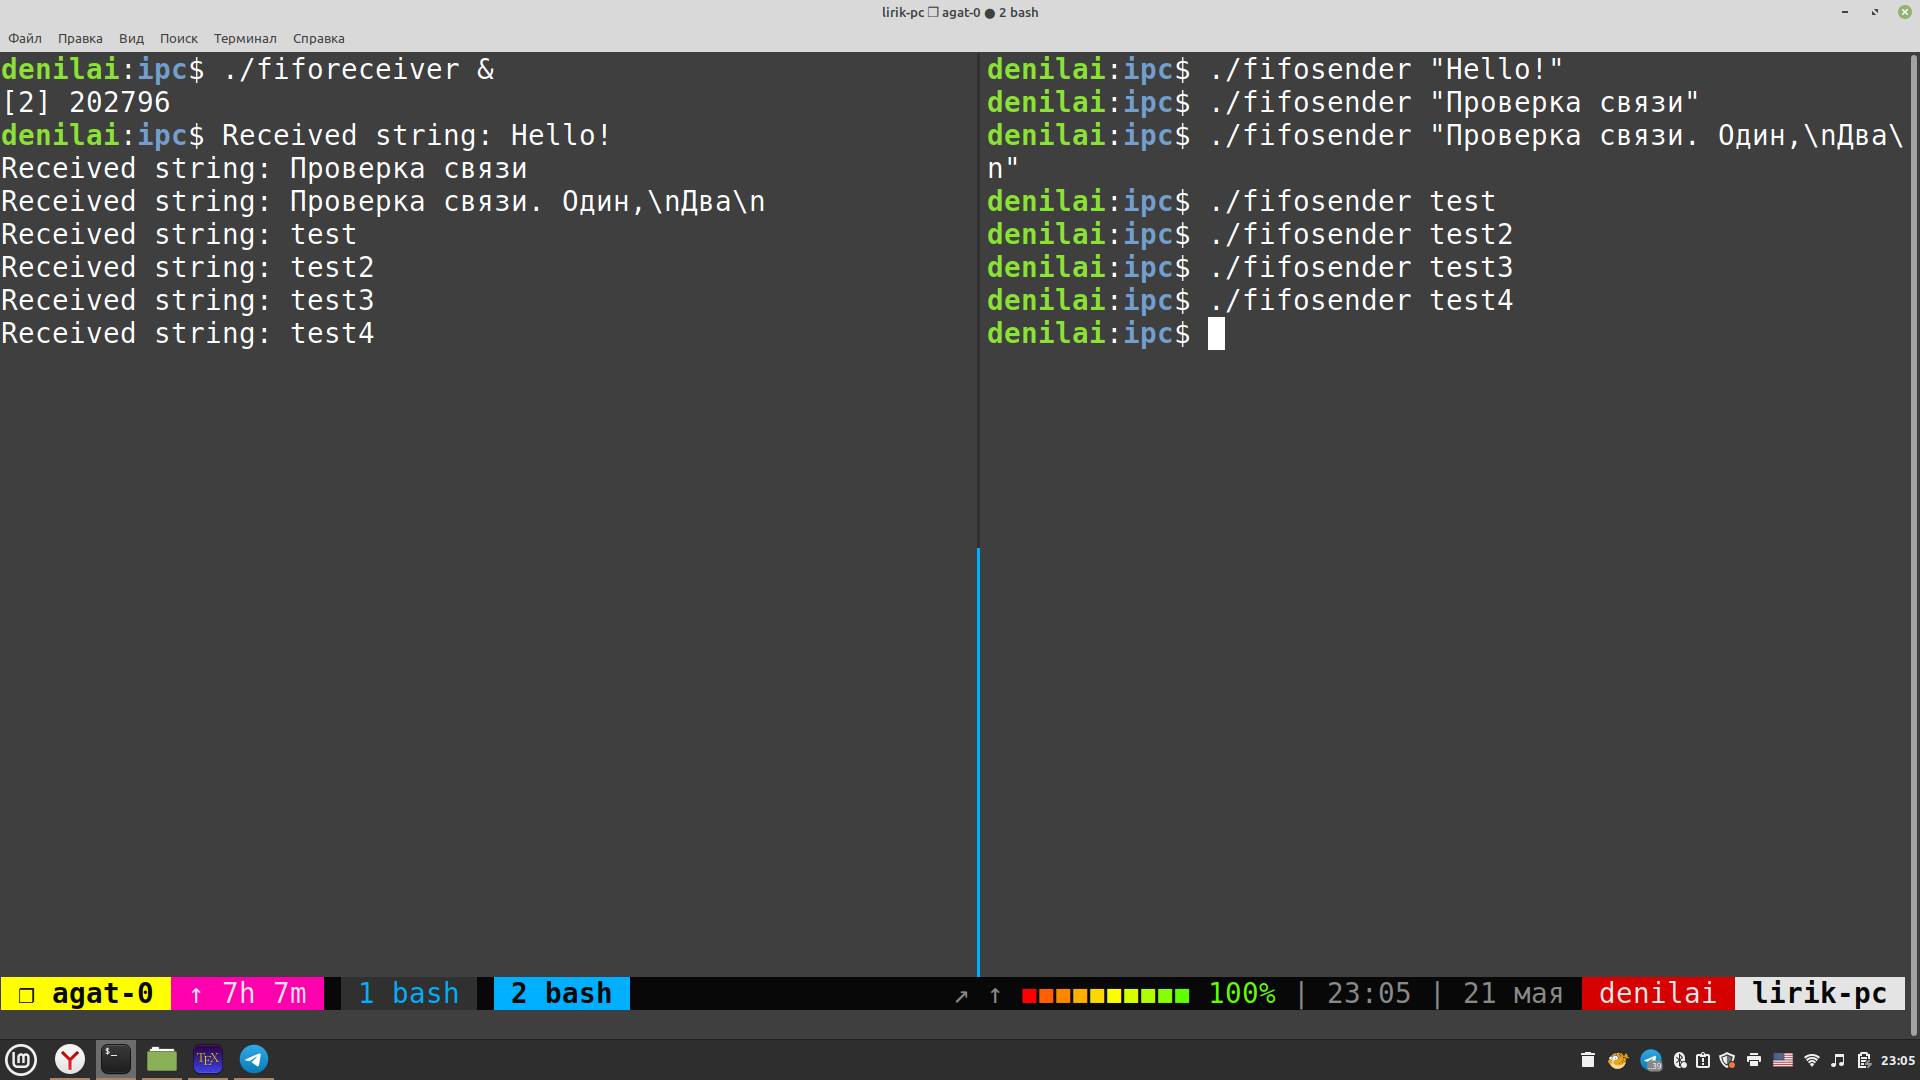
\includegraphics[width=0.9\linewidth]{images/6/demo}
	\caption{Вывод программ npipesender и npipereceiver}
	\label{fig:demo}
\end{figure}
\newpage
\subsection{Очереди сообщений}

Реализуем программу, в которой продемонстрируем организацию межпроцессного взаимодействия с помощью очередей сообщений System V API.

Напишем две программы --- msgsending.c и msgreceiving.c 

\begin{lstlisting}[language=C, caption={msgsending.c}, label={lst:msgs}]
	#include <signal.h>
	#include <sys/types.h>
	#include <sys/ipc.h>
	#include <sys/wait.h>
	#include <unistd.h>
	#include <sys/msg.h>
	#include <stdio.h>
	#include <string.h>
	#include <stdlib.h>
	
	#define MAXSIZE 128
	
	int msqid;
	void sigint_handler(int sig){
		printf("\n=== handle SIGINT ===\n");
		msgctl(msqid,IPC_RMID,NULL);
		exit (0);
	}
	
	typedef struct msgbuf {
		long mtype;
		char mtext[MAXSIZE];
	}msgbuf;
	
	int main()
	{
		struct sigaction sa;
		
		sa.sa_handler = sigint_handler;
		sa.sa_flags = 0;
		sigemptyset(&sa.sa_mask);
		if (sigaction(SIGINT, &sa, NULL) == -1){
		perror("sigaction");
		exit(1);
		}
		int msgflg = IPC_CREAT | 0666;
		key_t key;
		msgbuf sbuf;
		size_t buflen;
		key = ftok("/home/denilai/myFile", 'b');
		//key = 1234;
		
		if ((msqid = msgget(key, msgflg )) < 0)
		{
			perror("msgsnd");
			exit(1);
		}
		while (1)
		{
			sbuf.mtype = 1;
			//Message type
			printf("Get your message: ");
			scanf("%[^\n]",sbuf.mtext);
			getchar();
			buflen = strlen(sbuf.mtext) + 1;
			
			if (msgsnd(msqid, &sbuf, buflen, IPC_NOWAIT) < 0)
			{
				printf ("ERROR MESAGE SENDING\n"); perror("msgsnd");
				exit(1);
			}
			else printf("The message has been sent\n");
		}
		
		msgctl(msqid,IPC_RMID,NULL);
		exit(0);
	}
\end{lstlisting}

\newpage
\begin{lstlisting}[language=C, caption={msgreceive.c}, label={lst:msgs}]
#include <sys/types.h>
#include <sys/ipc.h>
#include <sys/msg.h>
#include <stdio.h>
#include <stdlib.h>
#define MAXSIZE 128

typedef struct msgbuf
{
	long mtype;
	char mtext[MAXSIZE];
} msgbuf;


int main()
{
	int msqid;
	key_t key;
	msgbuf rcvbuffer;
	
	//key = 1234;
	key = ftok("/home/aj/myFile", 'b');
	
	
	if ((msqid = msgget(key, 0666)) < 0)
	{
		perror("msgsnd");
		exit(1);
	}
	int byte_size;
	
	if ((byte_size = msgrcv(msqid, &rcvbuffer, MAXSIZE, 1, 0)) < 0)
	{
		perror("msgrcv");
		exit(1);
	}
	printf("%s\n", rcvbuffer.mtext);
	printf("Message size = %d\n",byte_size-1);
	exit(0);
}

\end{lstlisting}

Доступ к файлу осуществляется с помощью уникального ключа, в данном примере являющемся результатом функции ftok().

Если в очереди недостаточно свободного места, то функция msgsnd() по умолчанию блокируется до тех пор, пока свободное место не станет доступным. Если IPC\_NOWAIT указан в msgflg, то вызов вместо этого завершается ошибкой EAGAIN.

Настроим обработку сигналов аналогично прошлой лабораторной работе. Перед завершением, программа отправит команду на удаление очереди сообщений.


Если сообщение запрошенного типа недоступно и IPC\_NOWAIT не указан в msgflg, вызывающий процесс блокируется до тех пор, пока не возникнет одно из следующих условий:
\begin{itemize}
	\item сообщение нужного типа попадет в очередь;
	\item очередь сообщений будет удалена из системы. В этом случае системный вызов завершается ошибкой errno=EIDRM.
\end{itemize}

Продемонстрируем работу программы (см. рисунок \ref{fig:demo1}).
% TODO: \usepackage{graphicx} required
\begin{figure}[h!]
	\centering
	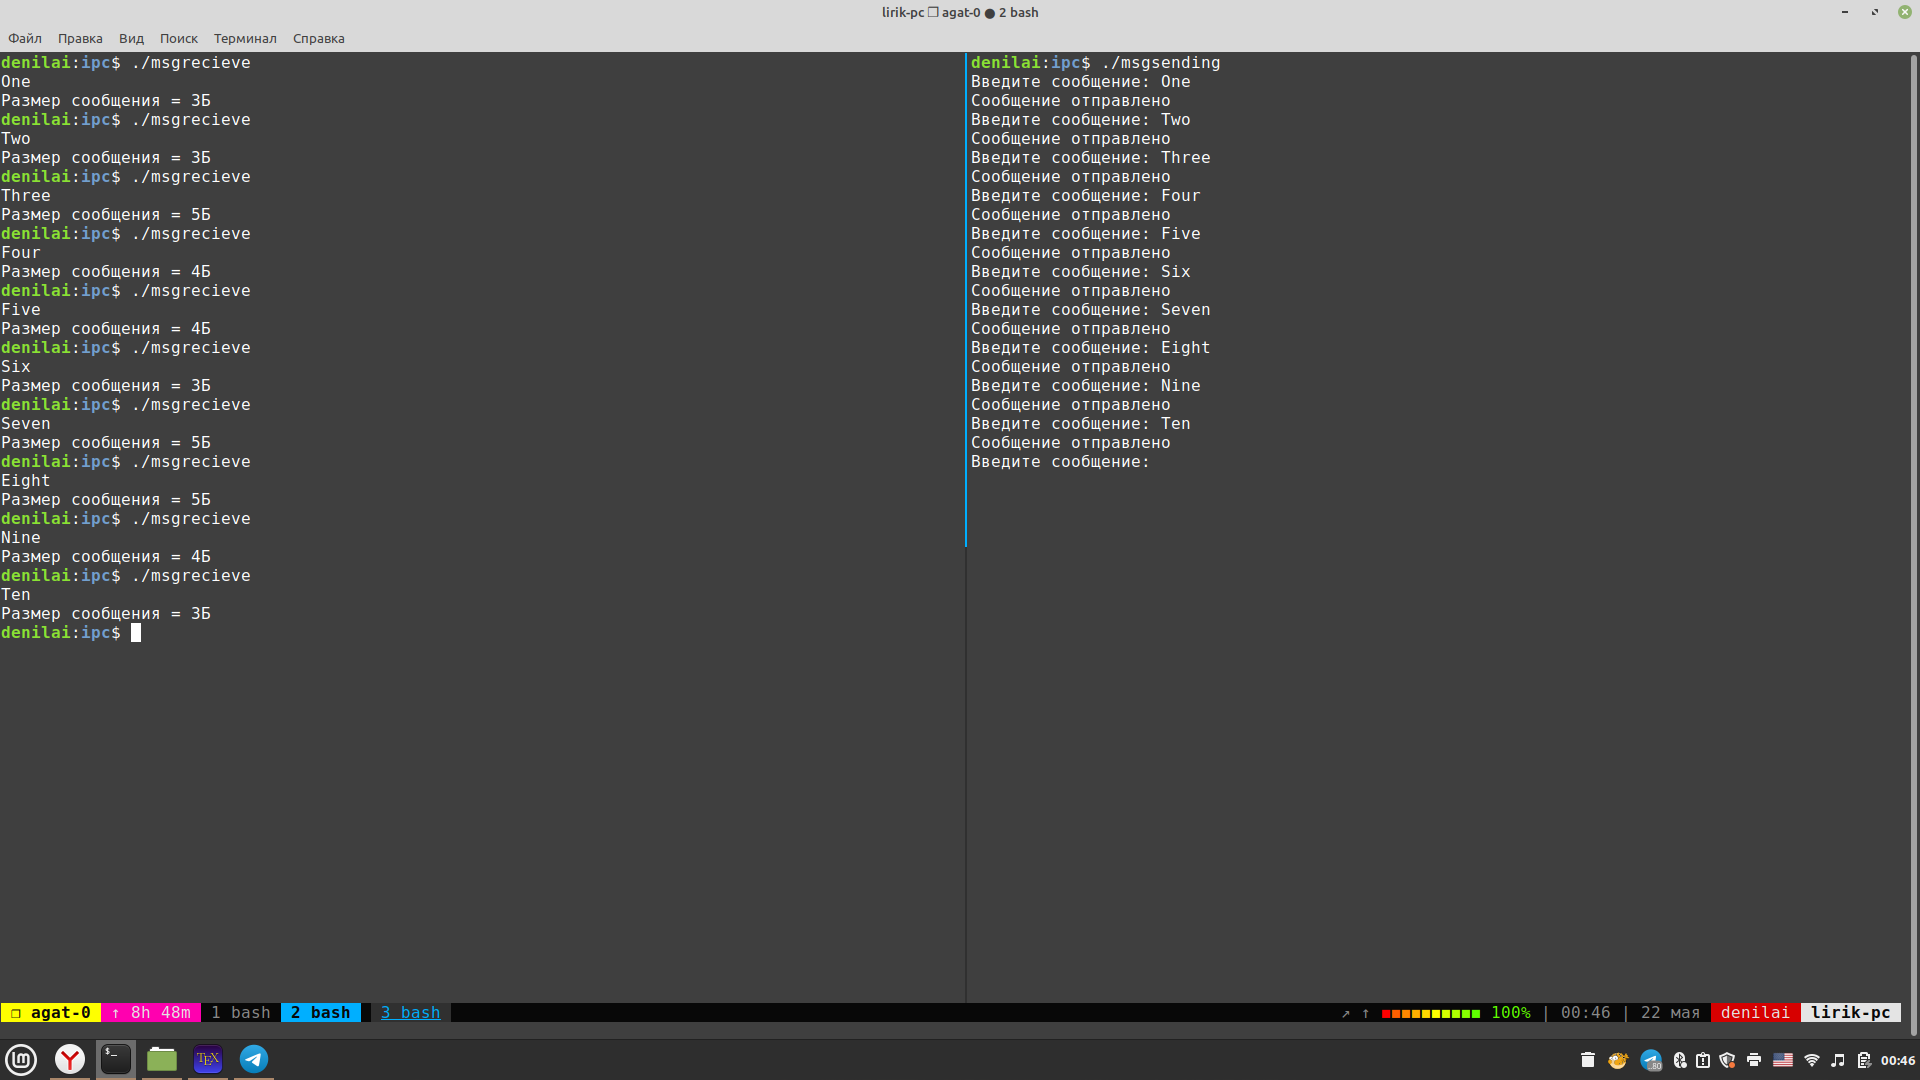
\includegraphics[width=0.9\linewidth]{images/6/demo1}
	\caption{Демонстрация работы очередей}
	\label{fig:demo1}
\end{figure}


\subsection{Общие сегменты памяти}

Разделяемая память является наиболее быстрым средством межпроцессного взаимодействия. После отображения области памяти в адресное пространство процессов, совместно ее использующих, для передачи данных между процессами больше не требуется участие ядра (процессы не делают системных вызовов для передачи данных). Обычно, однако, требуется некоторая форма синхронизации процессов, помещающих данные в разделяемую память и считывающих ее оттуда. 

Реализуем программу, демонстрирующую организацию межпроцессного взаимодействия с помощью общих сегментов памяти.

Напишем два файла --- memwrite.c и memwrite.c. В этих файлах опишем процесс выделения участка памяти, который будет использован двумя разными процессами. Будем использовать POSIX API для создания блоков памяти.


Функция mmap отображает в адресное пространство процесса файл или объект разделяемой памяти Posix. 
\begin{lstlisting}[language=C]
	#include <sys/mman.h>
	void *mmap(void *addr, size_t len, int prot, int flags, int fd, off_t offset);
	
\end{lstlisting}
	mmap() Возвращает начальный адрес участка памяти в случае успешного завершения. MAP\_FAILED – в случае ошибки.

 
 Защита участка памяти с отображенным объектом обеспечивается с помощью аргумента prot и констант, приведенных в табл. \ref{tab:prot}. Обычное значение этого аргумента — PROT\_READ | PROT\_WRITE, что обеспечивает доступ на чтение и запись.
 
 Таблица 12.1. Аргумент prot для вызова mmap
 
 
 \begin{table}[h!]
 	\centering
 	\caption{Аргумент prot для вызова mmap}
 	\begin{tabular}{|l|l|}
 		\hline
 		\textbf{prot} & \textbf{Описание} \\ \hline
 		PROT\_READ & Данные могут быть считаны \\ \hline
 		PROT\_WRITE & Данные могут быть записаны \\ \hline
 		PROT\_EXEC & Данные могут быть выполнены \\ \hline
 		PROT\_NONE & Доступ к данным закрыт \\ \hline
 	\end{tabular}
 	\label{tab:prot}
 \end{table}

Аргумент flags может принимать значения из табл. \ref{tab:flag} Можно указать только один из флагов — MAP\_SHARED или MAP\_PRIVATE, прибавив к нему при необходимости MAP\_FIXED. Если указан флаг MAP\_PRIVATE, все изменения будут производиться только с образом объекта в адресном пространстве процесса; другим процессам они доступны не будут. Если же указан флаг MAP\_SHARED, изменения отображаемых данных видны всем процессам, совместно использующим объект
 
 
 \begin{table}[h!]
 	\centering
 	\caption{Аргумент flag для вызова mmap}
 	\begin{tabular}{|l|p{0.6\linewidth}|}
 		\hline
 		\textbf{flag} & \textbf{Описание} \\ \hline
 		MAP SHARED & Изменения передаются другим процессам \\ \hline
 		MAP\_PRIVATE & Изменения не передаются другим процессам и не влияют на отображенный объект \\ \hline
 		MAP\_FIXED & Аргумент addr интерпретируется как адрес памяти \\ \hline
 	\end{tabular}
 	\label{tab:flag}
 \end{table}


\begin{lstlisting}
	#include <sys/mman.h>
	int shm_open(const char *name, int oflag, mode_t mode);
\end{lstlisting}
	shm\_open() возвращает неотрицательный дескриптор в случае успешного завершения, -1 – в случае ошибки.


\begin{lstlisting}

int shm_unlink(const char *name);

\end{lstlisting}
shm\_unlink() возвращает 0 в случае успешного завершения, -1 – в случае ошибки.

Аргумент oflag должен содержать флаг O\_RDONLY либо O\_RDWR и один из следующих: O\_CREAT, O\_EXCL, O\_TRUNC. Флаги O\_CREAT и O\_EXCL были описаны в разделе 2.3. Если вместе с флагом O\_RDWR указан флаг O\_TRUNC, существующий объект разделяемой памяти будет укорочен до нулевой длины.

Аргумент mode задает биты разрешений доступа (табл. 2.3) и используется только при указании флага O\_CREAT. Обратите внимание, что в отличие от функций mq\_open и sem\_open для shm\_open аргумент mode указывается всегда. Если флаг O\_CREAT не указан, значение аргумента mode может быть нулевым.

Возвращаемое значение shm\_open представляет собой целочисленный дескриптор, который может использоваться при вызове mmap в качестве пятого аргумента.

Функция shm\_unlink удаляет имя объекта разделяемой памяти.
 


Для отключения отображения объекта в адресное пространство процесса используется вызов munmap:

\begin{lstlisting}[language=C]
#include <sys/mman.h>
int munmap(void *addr, size_t len);

\end{lstlisting}
 munmap() возвращает 0 в случае успешного завершения, -1 --- в случае ошибки.
 
 Приведем листинг программ: 
 
\begin{lstlisting}[language=C, caption={memwrite.c}, label={lst:memw}]
#include <stdio.h>
#include <sys/mman.h>
#include <fcntl.h>
#include <unistd.h>
#include <string.h>

#define NUM 3
#define SIZE (NUM * sizeof(int))

#define FILE_PATH "/shared-segment"


int main(){
	int fd = shm_open(FILE_PATH, O_CREAT | O_EXCL | O_RDWR, 0600);
	if (fd < 0)
	{
		perror("shm_open()");
		return 0;
	}
	
	ftruncate(fd, SIZE);
	int *data = (int *) mmap(0, SIZE, PROT_READ | PROT_WRITE, MAP_SHARED,  fd, 0);
	printf("sender mapped address : %p\n",data);
	
	for (int i =0; i < NUM; i++){
		data[i] = i;
	}
	munmap(data, SIZE);
	close(fd);
	return 0;
}
\end{lstlisting}


\begin{lstlisting}[language=C, caption={memread.c}, label={lst:memr}]

#include <stdio.h>
#include <sys/mman.h>
#include <fcntl.h>
#include <unistd.h>
#include <string.h>

#define NUM 3
#define SIZE (NUM * sizeof(int))

#define FILE_PATH "/shared-segment"


int main(){
	int fd = shm_open(FILE_PATH, O_RDONLY, 0600);
	if (fd < 0)
	{
		perror("shm_open()");
		return 0;
	}
	
	int *data = (int *) mmap(0, SIZE, PROT_READ, MAP_SHARED,  fd, 0);
	printf("sender mapped address : %p\n",data);
	
	for (int i =0; i < NUM; i++){
		printf("%d\n", data[i]);
	}
	munmap(data, SIZE);
	close(fd);
	shm_unlink(FILE_PATH);
	return 0;
}
 \end{lstlisting}
 
 Продемонстрируем работы программ (см. рисунок \ref{fig:demo2}).
 
 
 % TODO: \usepackage{graphicx} required
 \begin{figure}[h!]
 	\centering
 	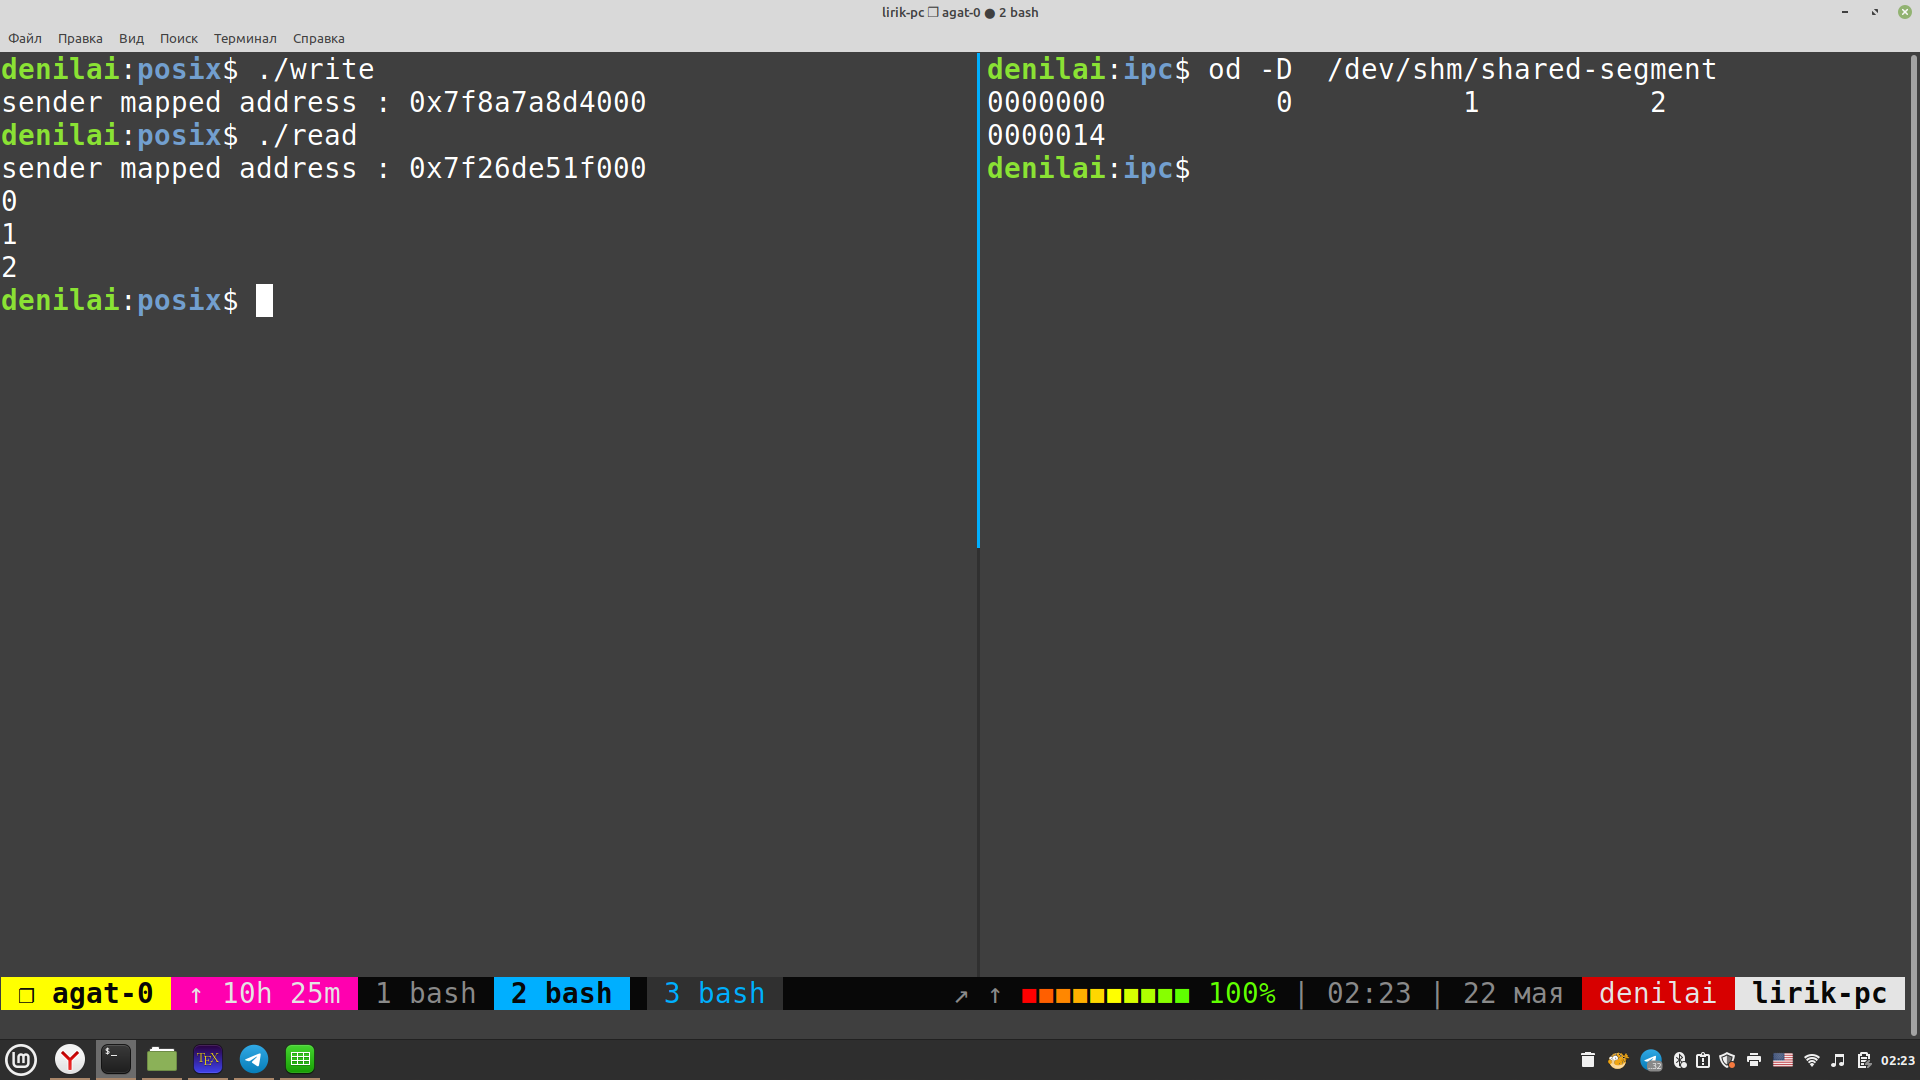
\includegraphics[width=0.9\linewidth]{images/6/demo2}
 	\caption{Демонстрация работы программ memwrite и memread}
 	\label{fig:demo2}
 \end{figure}
 


\clearpage
\section{Вывод}

В ходе настоящей лабораторной работы были созданы программы для демонстрации организации межпроцессного взаимодействия с помощью каналов, очередей сообщений, семафоров и сегментов общей памяти. Были использованы интерфейсы POSIX и System V. 


\end{document}

